\documentclass[10pt,a4paper]{article}

% ------------------------------------------------------------------
% Packages
% ------------------------------------------------------------------
\usepackage[utf8]{inputenc}
\usepackage[T1]{fontenc}
\usepackage{lmodern}
\usepackage{textcomp}
\usepackage[margin=1.8cm]{geometry}
\usepackage{graphicx}
\usepackage{booktabs}
\usepackage{tabularx}
\usepackage{caption}
\usepackage{subcaption}
\usepackage{enumitem}
\usepackage{xcolor}
\usepackage{titlesec}
\usepackage[hidelinks]{hyperref}

\graphicspath{{./}{figures/}}
\captionsetup{font=small,labelfont=bf,skip=4pt}
\setlist{nosep,leftmargin=*}
\setlength{\parskip}{3pt}
\setlength{\parindent}{0pt}
\titlespacing*{\section}{0pt}{8pt}{3pt}
\titlespacing*{\subsection}{0pt}{5pt}{2pt}
\titleformat{\section}{\large\bfseries\color{blue!50!black}}{\thesection.}{0.5em}{}
\titleformat{\subsection}{\normalsize\bfseries}{\thesubsection}{0.5em}{}

\newcommand{\eur}{\,\texteuro}

% ------------------------------------------------------------------
\begin{document}

\begin{center}
{\LARGE\bfseries Tasko: what really drives growth before the Series A?}\\[4pt]
{\large Growth Modeling \& Data-Driven Strategy --- Final project, IMT 2026}\\[2pt]
{Group [number] --- [Names]}
\end{center}

\vspace{-2pt}
\noindent\fcolorbox{blue!50!black}{blue!4}{\parbox{\dimexpr\textwidth-2\fboxsep-2\fboxrule}{
\textbf{Answer to the board.} Tasko's growth is genuinely product-led, but \emph{after} the sign-up rather than before it. A workspace that gathers a team of three converts 2.5 times more often, and the existing base feeds a guest loop that already brings one new workspace in five. Paid search, the largest marketing line, buys sign-ups at a constant price but few teams: its LTV\,:\,CAC is 1.2 on revenue and its payback 31 months. The onboarding change of September 2025 is the most consequential event of the period. Our model projects an MRR of 42 to 109\,k\eur{} in June 2027, and shows that conversion and team size matter far more than additional ad spend.
}}

% ==================================================================
\section{Data and method}

The analysis covers 18 months of activity (January 2025 -- June 2026), extracted on 30 June 2026. The four raw files were cleaned with explicit, counted rules; the full cleaning log is given in Table~\ref{tab:log}. Three definitions structure the study:
\begin{itemize}
  \item \textbf{Activation}: at least two teammates join the workspace within 30 days of its creation (justified in Section~2).
  \item \textbf{Conversion}: upgrade to a paid plan within 90 days. The longest observed delay being 89 days, only cohorts created before April 2026 are fully observed.
  \item \textbf{Churn}: a paying workspace whose last invoice predates June 2026. No gap was found in billing histories.
\end{itemize}
Since the data pack provides no gross margin, all lifetime values are \emph{revenue} LTVs ($\text{LTV} = \text{ARPA}/\text{churn}$), and should be read as upper bounds.

% ==================================================================
\section{Funnel and growth loop}

\textbf{Activation is the hinge of the funnel.} Conversion stays at 5--6\,\% for workspaces with zero or one teammate, then more than doubles from two teammates onwards (12.5\,\%) and keeps rising to 17.7\,\% beyond six (Figure~\ref{fig:funnel}, right). The threshold is sharp enough to serve as the \emph{Aha moment} of the AARRR framework: a team of three.

\begin{figure}[h]
  \centering
  \begin{subfigure}{0.53\textwidth}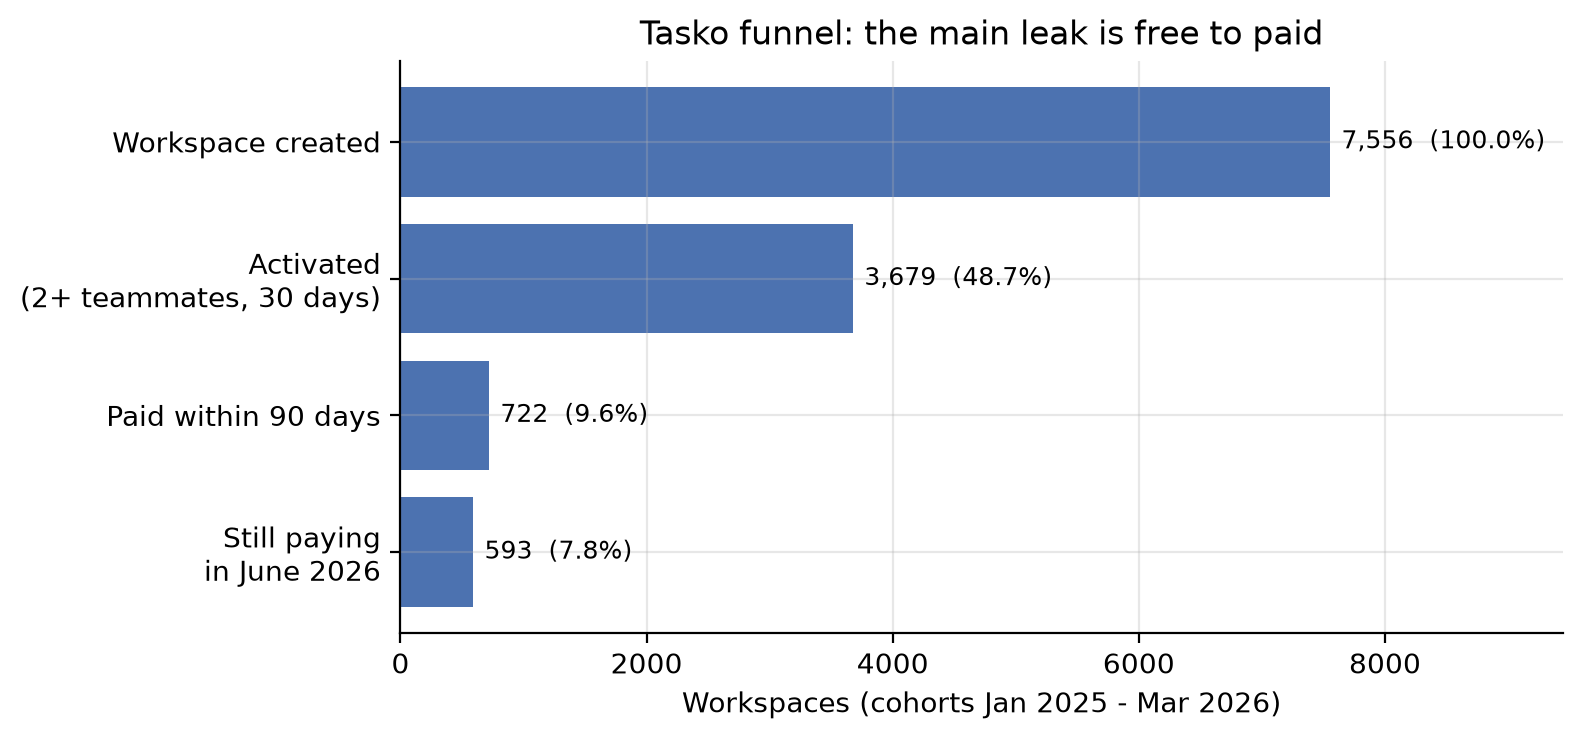
\includegraphics[width=\linewidth]{fig02_funnel.png}\end{subfigure}\hfill
  \begin{subfigure}{0.45\textwidth}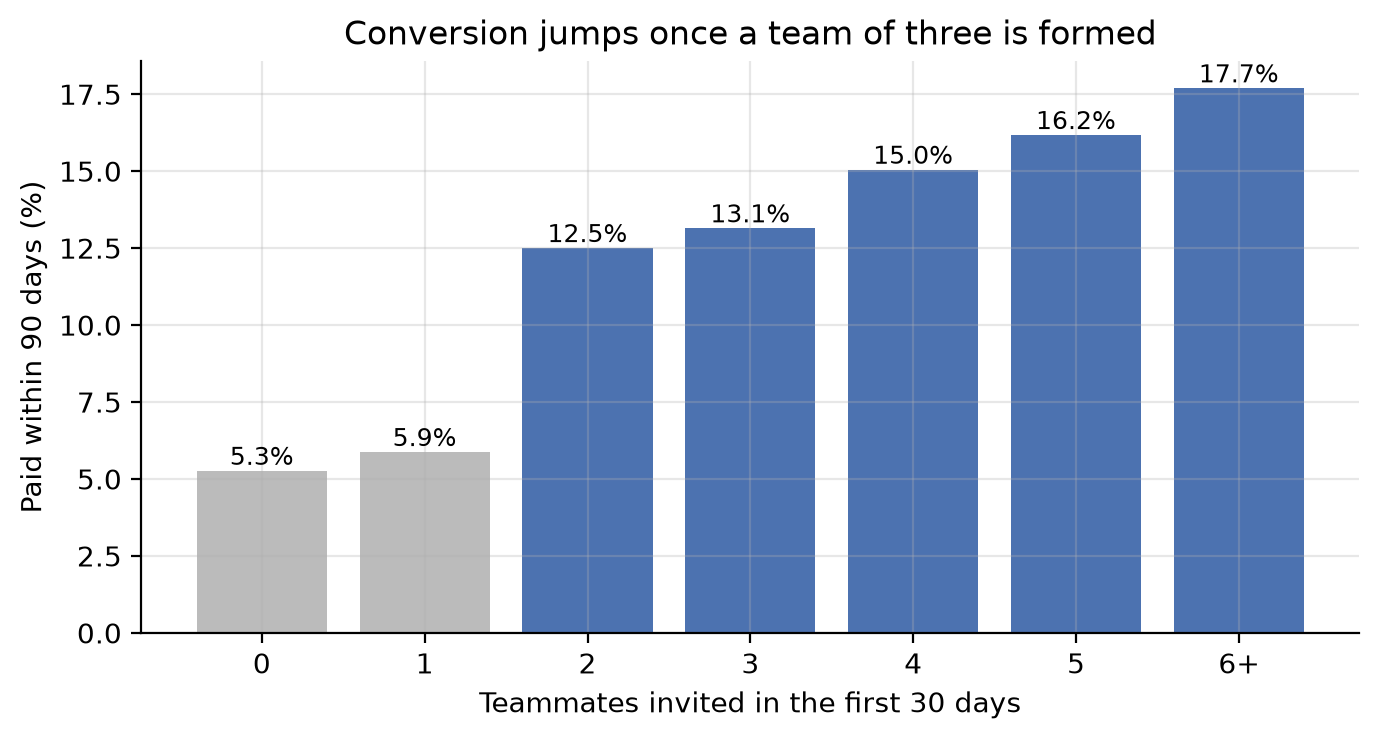
\includegraphics[width=\linewidth]{fig01_aha_moment.png}\end{subfigure}
  \caption{Funnel of the cohorts January 2025 -- March 2026 (left) and 90-day conversion by number of teammates invited in the first month (right).}
  \label{fig:funnel}
\end{figure}

Of 7,556 workspaces, 48.7\,\% are activated, 9.6\,\% pay within 90 days and 7.8\,\% still pay in June 2026. Once a workspace pays, it largely stays (82\,\%). \textbf{Value therefore leaks at the free-to-paid step}, and activation governs that leak: activated workspaces convert at 13.8\,\% against 5.6\,\%, and account for 70\,\% of all conversions.

\textbf{A real but modest loop.} Guests of a workspace later create their own (\texttt{invite\_loop}). This channel rises from 0\,\% of new workspaces in January 2025 to 19.8\,\% in June 2026. The data does not record the invitations sent, so instead of $K = i \times c$ we measure the \emph{effective} virality: each workspace generates 0.09 new workspaces within 180 days before mid-September 2025, and 0.12 after. With $K \ll 1$, the loop does not replace acquisition; it multiplies it. It is also slow (median delay of 146 days), and, notably, its rate does not depend on the activation, payment or channel of the origin workspace. The loop is fed by the \emph{size} of the base, which is precisely why it compounds.

% ==================================================================
\section{Channels and segments}

Paid search lags on every early indicator: an activation of 29\,\% against 50--59\,\% elsewhere, a 90-day conversion of 6.4\,\% against 10.7--11.8\,\% for organic, SEO and loop, and smaller teams (3.1 seats, 27\eur{} ARPA against 35--38\eur).

\begin{figure}[h]
  \centering
  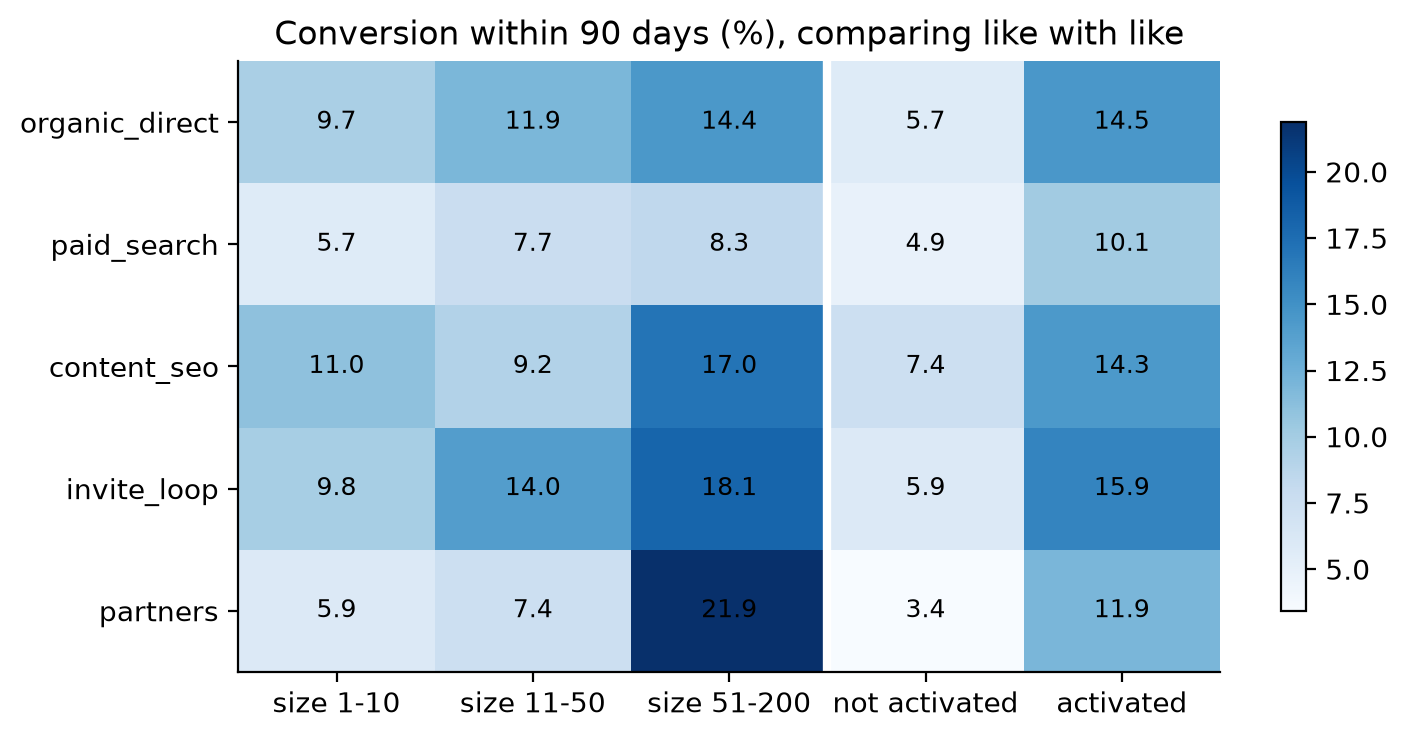
\includegraphics[width=0.66\textwidth]{fig06_like_for_like.png}
  \caption{90-day conversion (\%) by channel, within company size and within activation status.}
  \label{fig:lfl}
\end{figure}

\textbf{The gap survives a like-for-like comparison} (Figure~\ref{fig:lfl}). The size mix is nearly identical across channels (about 60\,/\,29\,/\,9\,\%), so composition cannot explain it, and paid search converts least within every size. Even among activated workspaces, it converts at 10.1\,\% against 14--16\,\% for organic, SEO and loop: its users are less likely to form a team, and less likely to pay once they have. The other channels are close to one another once like is compared with like.

Company size is the strongest driver of value. Workspaces of 51--200 employees hold 7 seats, bring 66\eur{} per month and churn at 1.2\,\% monthly, against 2.6 seats, 21\eur{} and 4.4\,\% for teams of 1--10. Business plans churn less than Pro (2.1\,\% vs 3.5\,\%).

% ==================================================================
\section{Unit economics}

\begin{table}[h]
\centering\small
\begin{tabular}{lrrrrrr}
\toprule
Channel & Cost per sign-up & CAC (paying) & ARPA & Monthly churn & LTV & LTV\,:\,CAC \;/\; payback \\
\midrule
Paid search  & 55\eur & 864\eur   & 27.5\eur & 2.7\,\% & 1,007\eur & 1.16 \;/\; 31.5 months \\
Content SEO  & 40\eur & 357\eur   & 37.8\eur & 3.7\,\% & 1,022\eur & 2.86 \;/\; 9.5 months \\
Partners     & 93\eur & 1,210\eur & 38.2\eur & 4.6\,\% & 830\eur   & 0.69 \;/\; 31.7 months \\
\bottomrule
\end{tabular}
\caption{Unit economics of the paid channels (cohorts January 2025 -- March 2026). Organic direct and invite loop carry no spend.}
\label{tab:ue}
\end{table}

Content SEO approaches the 3\,:\,1 benchmark with a payback under ten months, and its cost per sign-up falls from 50\eur{} to 29\eur{} over the period: the SEO flywheel, slow to build and compounding afterwards. Paid search is borderline: an LTV\,:\,CAC of 1.2 \emph{on revenue} would fall below 1 once any gross margin is applied, and its payback exceeds the observed lifetime of most cohorts. Its budget nearly doubled ($\times$1.95) while the cost per sign-up stayed at 55\eur: growth from this channel is linear in spend, a funnel that needs constant fuel. Partners destroy value (0.69). Because half of the paying workspaces arrive at no acquisition cost, the blended CAC is 302\eur, against 642\eur{} for paid channels alone.

Retention is sound: monthly churn averages about 3\,\%, logo retention lies between 76\,\% and 94\,\% after six months, and recent cohorts retain no worse than older ones. The six-month net revenue retention of the December 2025 base is 95\,\%: seat expansion of surviving accounts does not offset churn, so the rise of ARPA from 31.6\eur{} to 37.5\eur{} in the first half of 2026 comes mainly from new accounts arriving with larger teams.

% ==================================================================
\section{What changed, and what it caused}

\begin{figure}[h]
  \centering
  \begin{subfigure}{0.47\textwidth}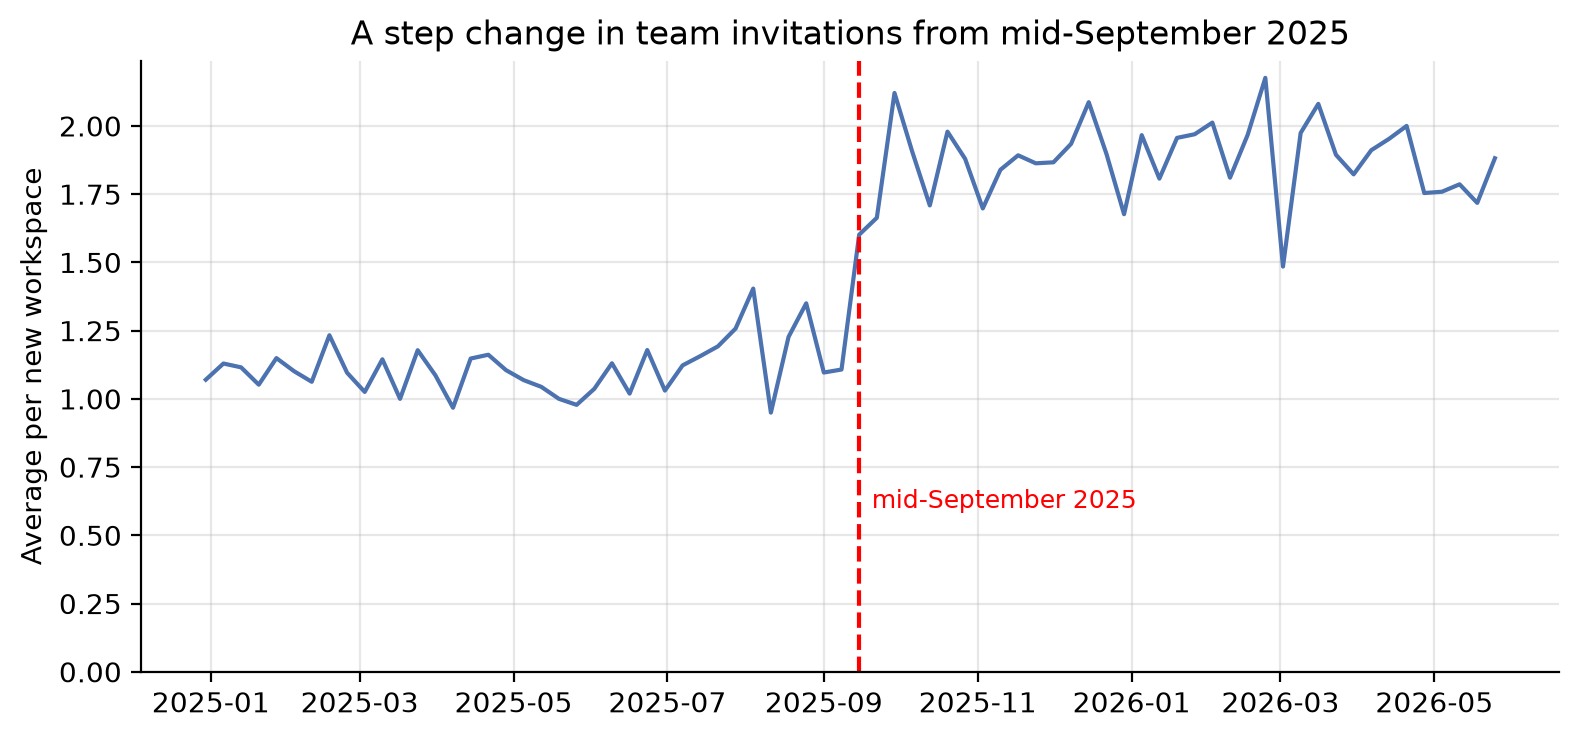
\includegraphics[width=\linewidth]{fig11_change_detection.png}\end{subfigure}\hfill
  \begin{subfigure}{0.51\textwidth}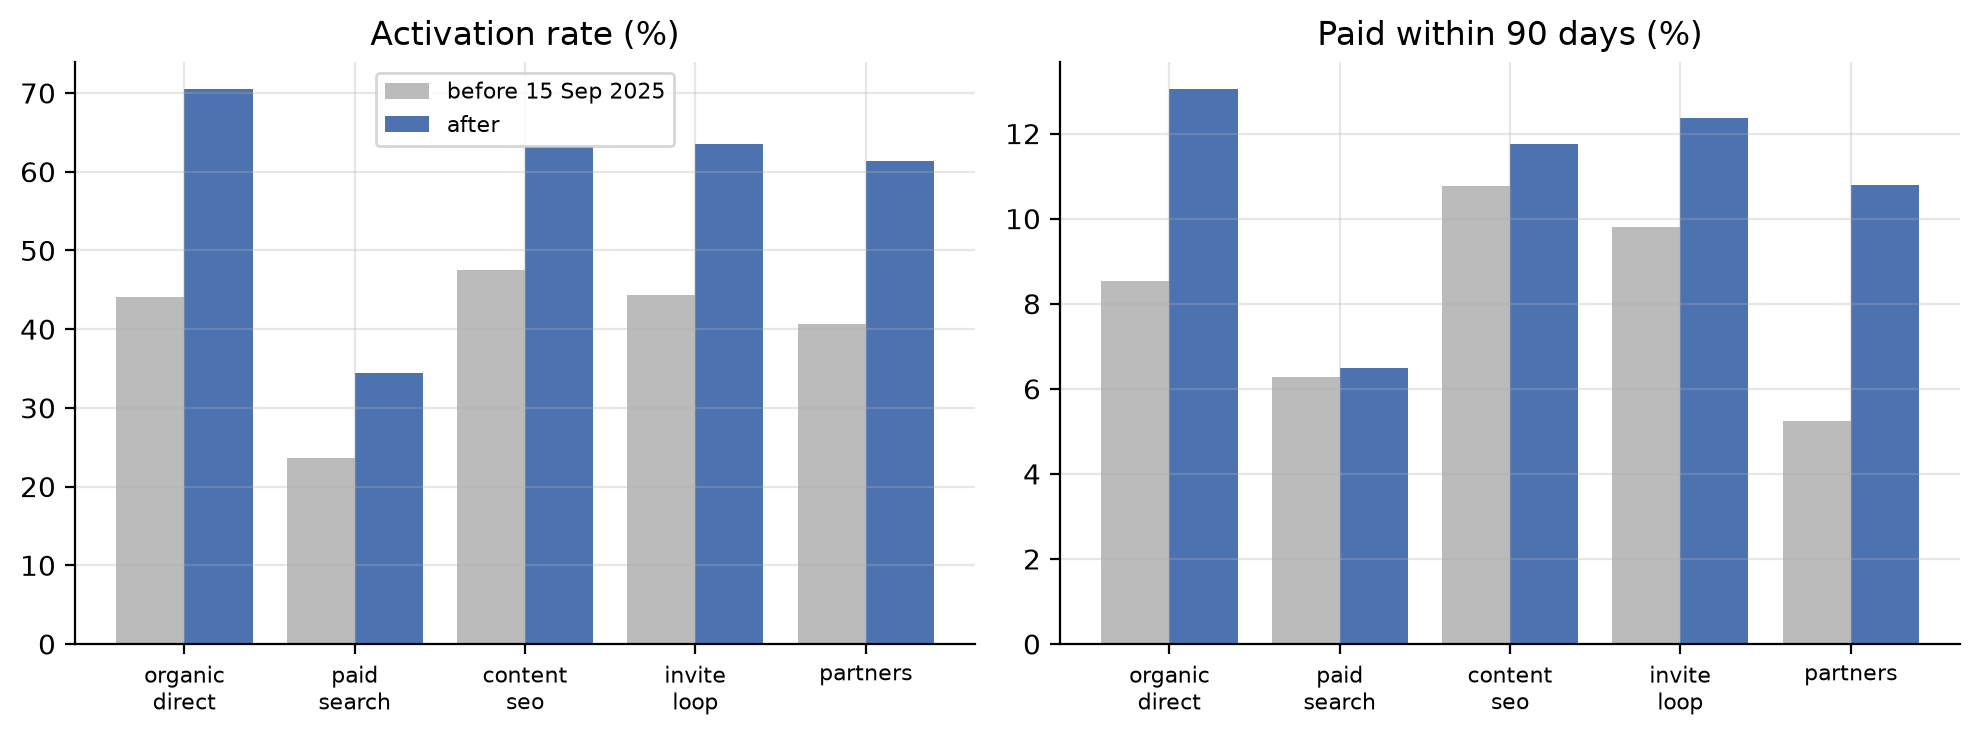
\includegraphics[width=\linewidth]{fig12_before_after.png}\end{subfigure}
  \caption{Teammates invited in the first week, by creation week (left); activation and conversion before and after 15 September 2025 (right).}
  \label{fig:change}
\end{figure}

In the second half of September 2025, the number of teammates invited during the first week of a workspace jumps from about 1.1 to about 1.9, and stays there (Figure~\ref{fig:change}). The data does not name the cause, but the shape --- a permanent step, across all channels --- points to an onboarding change rather than to a campaign. Its effects are clear: activation rises from 38\,\% to 58\,\%, 90-day conversion from 8.1\,\% to 10.8\,\%, and the effective K from 0.086 to 0.123, while churn is unaffected (3.2\,\% vs 3.3\,\%). The improvement holds within channel and size in 13 of the 15 cells, so it reflects a change of behaviour rather than of mix. \textbf{Paid search is the exception}: its activation rises far less (24\,\% $\rightarrow$ 35\,\%) and its conversion does not move (6.3\,\% $\rightarrow$ 6.5\,\%).

% ==================================================================
\section{North Star Metric}

We recommend \textbf{the number of workspaces reaching a team of three users each month} (about 600 in mid-2026). It captures the core value of a collaboration tool; it predicts revenue, since such teams convert 2.5 times more and Tasko bills per seat; it feeds the guest loop; and, unlike sign-ups, it cannot be inflated by paid spend alone. To avoid tunnel vision, it should be read with two guardrails: paid conversion and the churn of paying workspaces. With usage data, a stronger version would be \emph{weekly active teams of three or more}.

% ==================================================================
\section{Growth model, backtest and scenarios}

The model is monthly and follows the input\,/\,parameter\,/\,output structure seen in class. New workspaces are the sum of spend divided by the cost per sign-up of each paid channel, an organic trend, and a loop term (loop rate $\times$ existing base). New paying workspaces equal the conversion rate applied to past cohorts with the observed billing delay (one to four months); paying workspaces decay with monthly churn, and $\text{MRR} = \text{paying} \times \text{ARPA}$.

\begin{figure}[h]
  \centering
  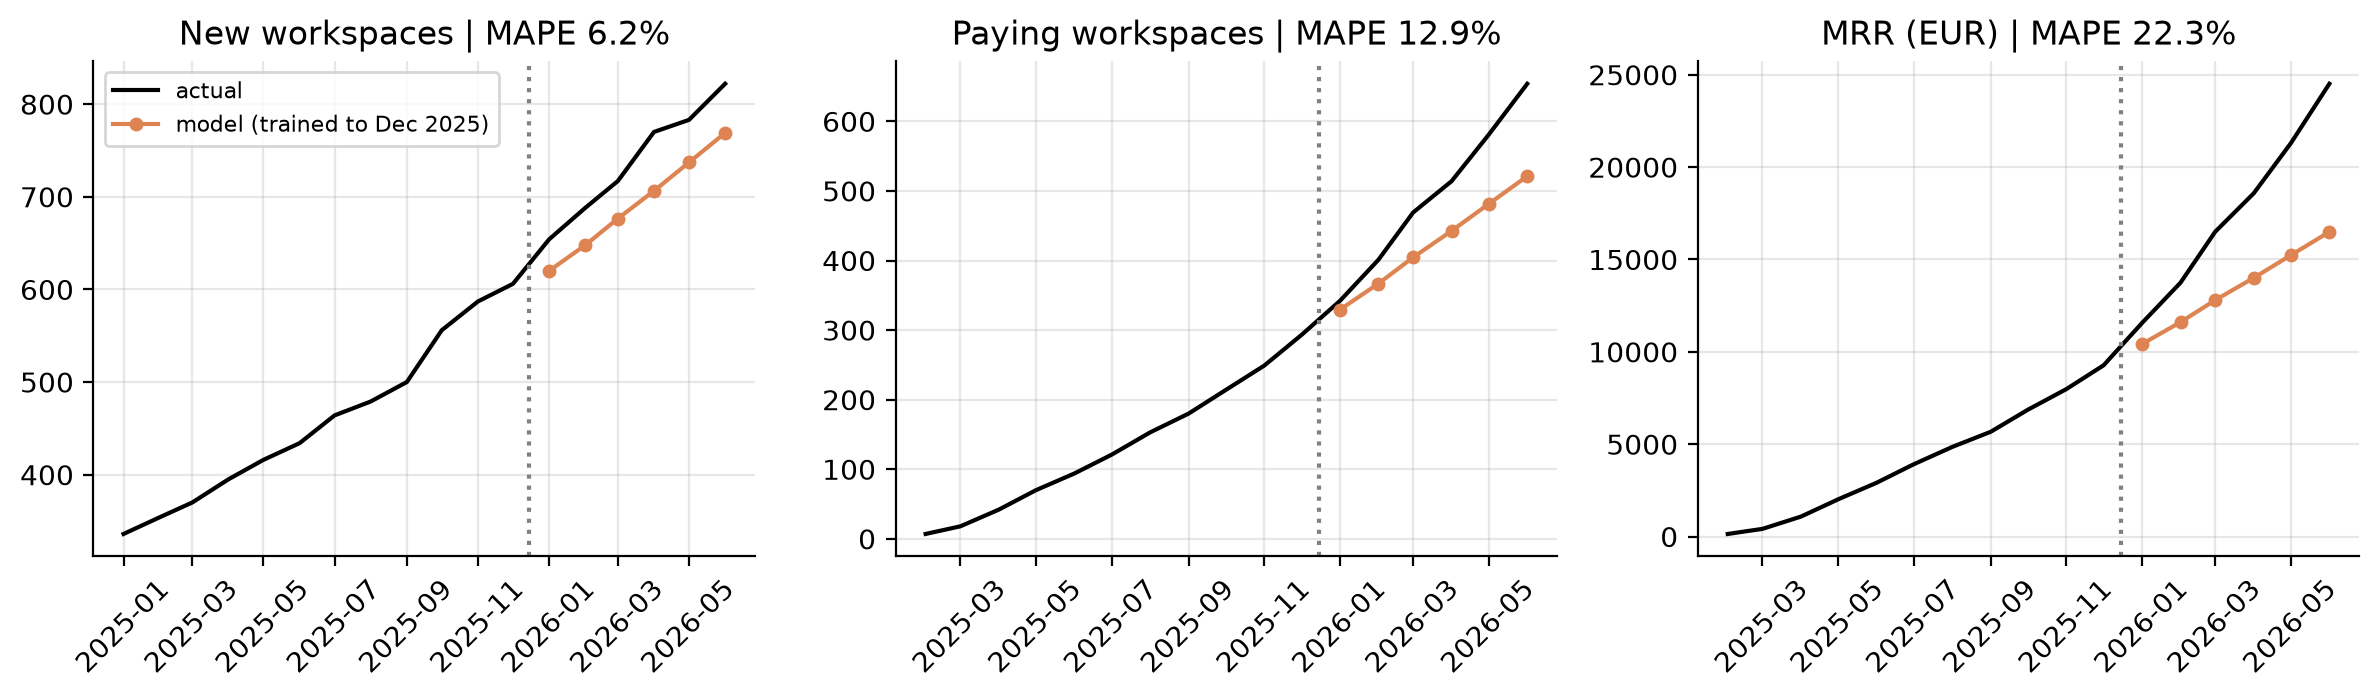
\includegraphics[width=\textwidth]{fig14_backtest.png}
  \caption{Backtest: model calibrated on data up to December 2025, run on January -- June 2026 with the actual spend.}
  \label{fig:bt}
\end{figure}

\textbf{Backtest.} Calibrated only on data available on 31 December 2025, the model predicts acquisition well (MAPE 6.2\,\%), but underestimates paying workspaces (12.9\,\%) and MRR (22.3\,\%), with an error that widens over time (Figure~\ref{fig:bt}). The decomposition is instructive: in December 2025 the onboarding change was too recent to show in mature cohorts. Using the post-change conversion brings the error on paying workspaces down to 4.0\,\%, and adding the observed 2026 ARPA brings the MRR error down to 6.2\,\%. The model is fragile exactly where the business changed.

\begin{figure}[h]
  \centering
  \begin{subfigure}{0.5\textwidth}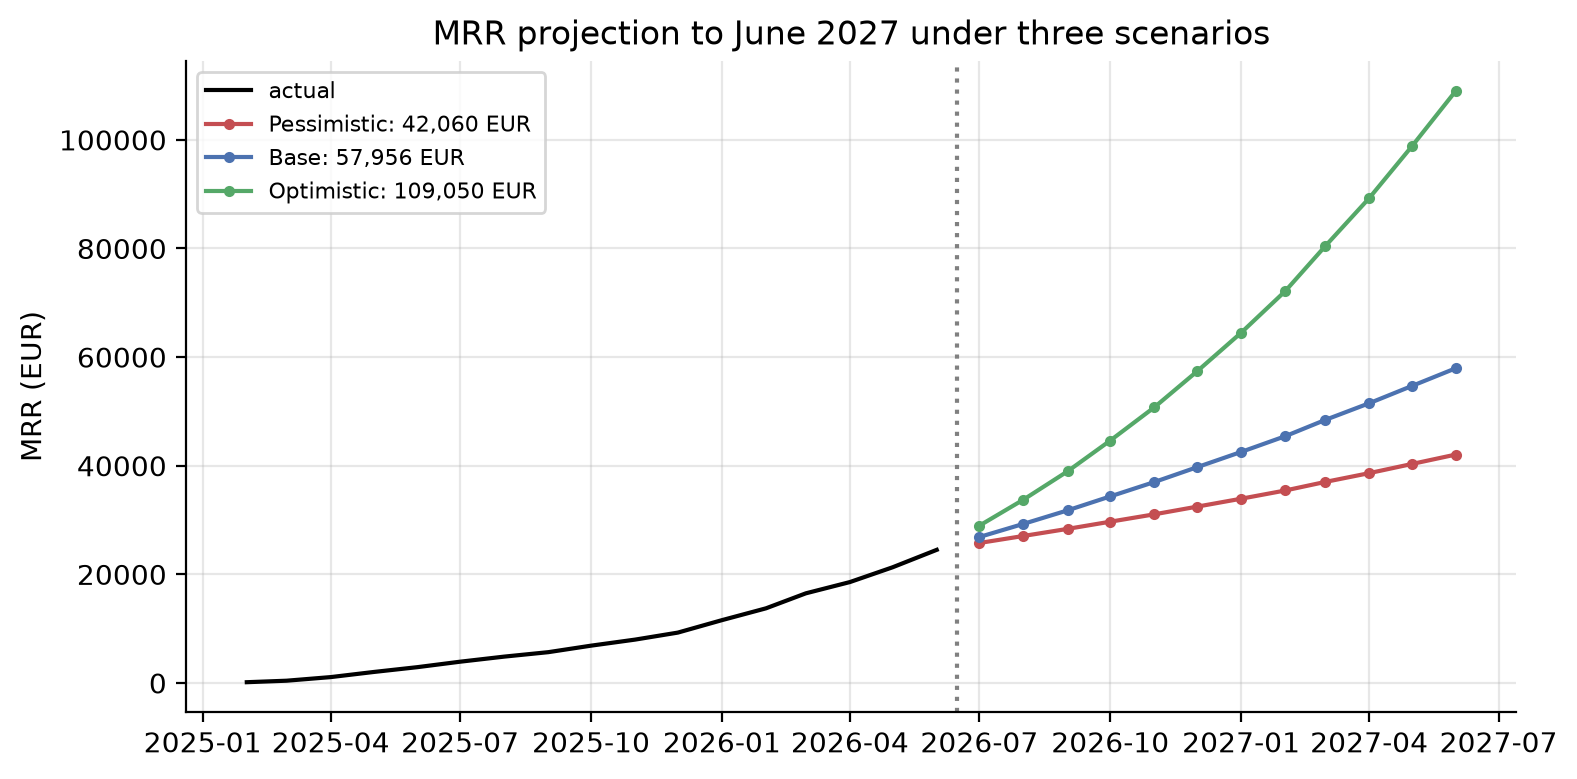
\includegraphics[width=\linewidth]{fig15_scenarios.png}\end{subfigure}\hfill
  \begin{subfigure}{0.48\textwidth}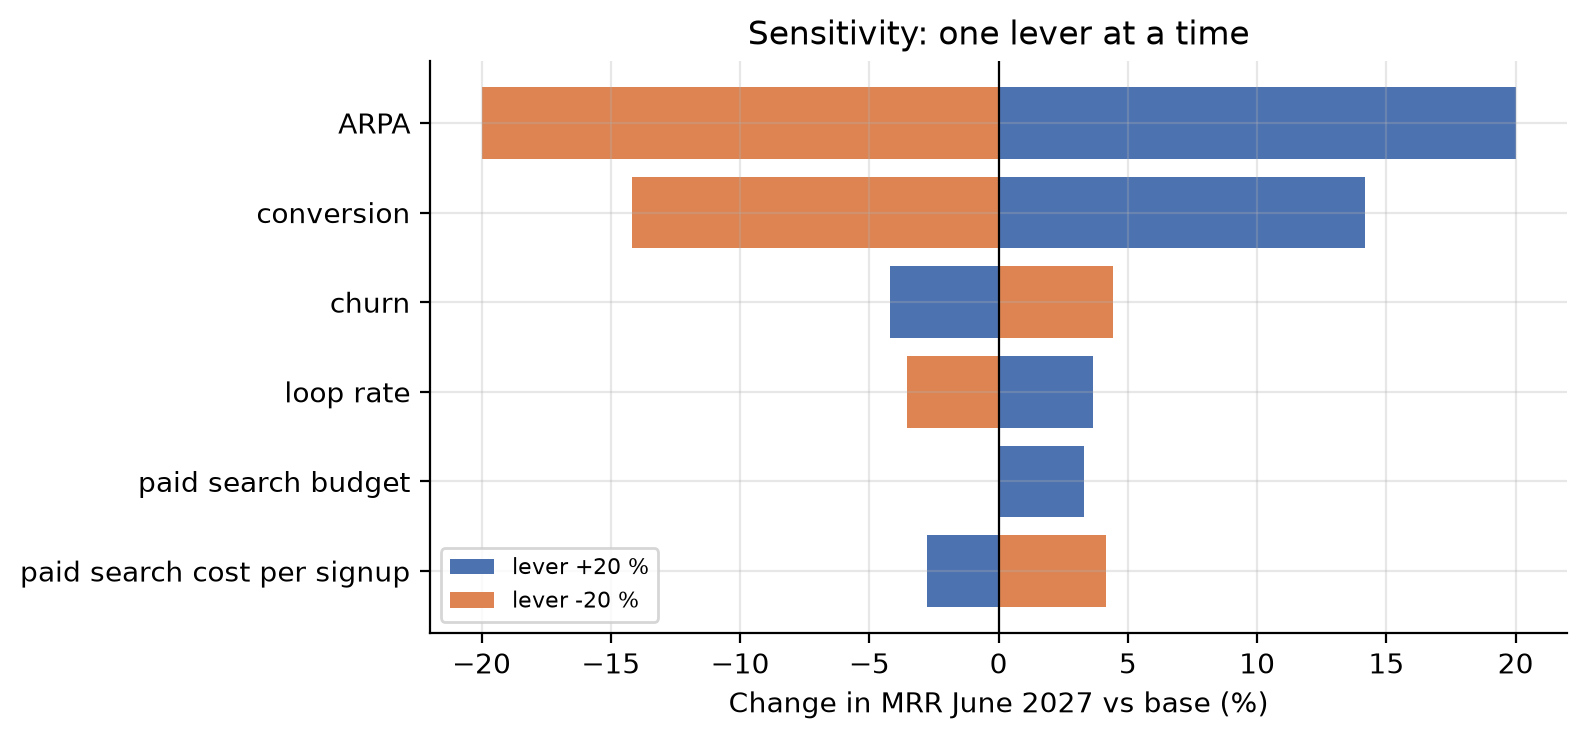
\includegraphics[width=\linewidth]{fig16_sensitivity.png}\end{subfigure}
  \caption{MRR projection under three scenarios (left) and sensitivity of June 2027 MRR to each lever moved by $\pm$20\,\% (right).}
  \label{fig:sc}
\end{figure}

\textbf{Scenarios (July 2026 -- June 2027).} All three scenarios share the current spend trends; each lever takes a value \emph{observed} in the data. The \emph{pessimistic} case returns to the pre-change conversion (8.1\,\%), the churn of small teams (4.4\,\%) and the pre-change loop rate (1.7\,\%). The \emph{base} case keeps the post-change conversion (10.8\,\%), churn (3.1\,\%) and loop rate (2.0\,\%). The \emph{optimistic} case uses the conversion of activated workspaces (14.4\,\%), the churn of Business plans (2.1\,\%), the best loop month (2.2\,\%) and the ARPA trend of the first half of 2026. June 2027 MRR reaches 42\,k\eur, 58\,k\eur{} and 109\,k\eur{} respectively (ARR of 0.50, 0.70 and 1.31\,M\eur). Strikingly, new workspaces barely differ (12.5\,k to 13.5\,k): the outcome is decided \emph{after} the sign-up. The sensitivity analysis confirms it: a 20\,\% lift in conversion adds 14\,\% of MRR, whereas 20\,\% more paid search budget adds only 3.3\,\%.

% ==================================================================
\section{A/B test plan}

\textbf{Hypothesis.} A guided, optional \emph{invite two teammates} step shown to paid search sign-ups before their first project will raise their activation, and in turn their conversion.
\begin{itemize}
  \item \textbf{Population and design}: new paid search workspaces, randomised 50/50 at creation.
  \item \textbf{Primary metric}: activation (2+ teammates within 30 days), baseline 34.5\,\%. \textbf{Secondary}: paid within 90 days (baseline 6.5\,\%). \textbf{Guardrails}: churn of paying workspaces, seats per workspace.
  \item \textbf{Sizing}: two-sided test on two proportions, $\alpha = 5\,\%$, power 80\,\%. With 204 paid search sign-ups per month, a minimum detectable effect of 8 points requires 577 workspaces per arm, i.e. about six months. A 5-point effect would need 14 months, and a test powered on a 2-point lift of conversion more than two years; activation is therefore the right primary metric. The September 2025 change lifted paid search activation by 11 points, which makes an 8-point effect plausible.
  \item \textbf{Ethics}: the step must remain optional and transparent --- no forced sharing, no automatic invitation of contacts.
\end{itemize}

% ==================================================================
\section{Recommendations}

\begin{enumerate}
  \item \textbf{Make the team of three the North Star}, and judge every initiative by its effect on it.
  \item \textbf{Cap paid search} at its current level until the A/B test shows that its users can be activated; redirect the increment to content SEO, the only paid channel near 3\,:\,1.
  \item \textbf{Renegotiate or stop partners}, whose LTV\,:\,CAC is below 1.
  \item \textbf{Invest in activation and team expansion}: they drive conversion, ARPA and the loop at once.
\end{enumerate}

% ==================================================================
\begin{table}[h]
\centering\footnotesize
\begin{tabularx}{\textwidth}{llXrl}
\toprule
\# & Table & Rule & Rows & Action \\
\midrule
1  & workspaces & Internal account (\texttt{W\_INTERNAL}, channel \texttt{internal}) & 1 & removed \\
2  & workspaces & Inconsistent \texttt{company\_size} labels (\texttt{1–10}, \texttt{11 to 50}, \texttt{11–50}) & 859 & harmonised \\
3  & workspaces & Missing \texttt{company\_size} & 267 & set to \texttt{unknown} \\
4  & workspaces & \texttt{invite\_loop} workspace created before its origin workspace & 66 & kept, excluded from loop timing \\
5  & users & Exact duplicate rows & 474 & removed \\
6  & users & Users of the internal workspace & 140 & removed \\
7  & users & \texttt{joined\_date} in DD/MM/YYYY format & 956 & converted \\
8  & users & Inviter not found in the users table & 1,591 & kept (membership valid) \\
9  & revenue & Exact duplicate rows & 22 & removed \\
10 & revenue & Negative MRR, always equal to $-$seats $\times$ price (sign error) & 25 & absolute value \\
11 & revenue & Upgraded workspaces without invoice (all upgraded in June 2026; first invoice always the following month) & 76 & kept \\
12 & all & Checks with no violation: upgrade before creation or after extraction, plan/date mismatch, duplicate \texttt{user\_id}, user joined before workspace or after extraction, double billing, MRR $\neq$ seats $\times$ price, revenue of free workspace, invalid spend & 0 & check only \\
\bottomrule
\end{tabularx}
\caption{Cleaning log. Final tables: 9,931 workspaces, 47,287 users, 4,402 invoices, 54 spend lines.}
\label{tab:log}
\end{table}

\end{document}
